\chapter{Relatively Brief \LaTeX{} Tutorial}
\label{ch:tutorial}

In this chapter, we will go through the basic elements of \LaTeX{} typesetting you may need for your thesis.
If you are reading this chapter already rendered in the PDF, make sure to also follow its source code located in
\verb|sections/chapter.tex|.

Before we start, this template provides two basic commands to make your life a bit easier: \verb|\todo| and
\verb|tocite|. You can use \todo\dots well, as a TO DO marker, and you can also use its parametrized version
\verb|\todo[something I have to do]| to leave comments for your future self. Similarly, you can \tocite to mark
places, where you would like to add some references later.

\section{Sectioning}
\label{sec:sectioning}

One of the most automatic aspects of \LaTeX{} is sectioning. At the top level, there are chapters, each
automatically starting on a new page with a large header. You can start a new chapter anywhere by
\verb|\chapter{Chapter Name}|. Chapters can be split into sections (via \verb|\section{Section Name}|) and further
into:

\subsection{Subsections}

This text belongs to a numbered subsection.

\subsubsection{Subsubsections}

This text belongs to a numbered subsubsection.

\paragraph{Labeled Paragraphs} This humble paragraph belongs to the subsubsection above. Note that the
paragraph name is inline, rather than on its own line: \emph{While questing once in noble wood of gray
medieval pine, I came upon a tomb, rain-slicked, rubbed cool, ethereal; its inscription long vanished,
yet still within its melancholy fissures --}

Note that all sections that are numbered automatically are also present in the table of contents. While this
template allows numbering down to subsubsections, it is generally not recommended to number them, as they tend to
fraction the document too much. Paragraphs are also never numbered. If you would like to use headings without
numbering, each of these commands has a starred version, which disables numbering and prevents the section from
appearing in the table of contents:

\subsection*{Unnumbered Subsection}

This text belongs to an unnumbered subsection.

\subsubsection*{Unnumbered Subsubsection}

This text belongs to an unnumbered subsubsection.


\section{Hyperlinking}
\label{sec:hyperlinks}

In your thesis, you should link your sections, figures, tables, and equations together so readers can easily jump
between different contexts. In \LaTeX{}, this is done by assigning a label \verb|\label{identifier}|
to individual elements.

For instance, this section is labeled with \verb|\label{sec:hyperlinks}|. It is best practice to use standardized
prefixes for your identifiers to keep your source code organized:
\begin{itemize}
    \item \verb|ch:| for chapters (e.g., \verb|ch:tutorial|)
    \item \verb|sec:| for sections and subsections (e.g., \verb|sec:hyperlinks|)
    \item \verb|fig:| for figures (e.g., \verb|fig:example|)
    \item \verb|tab:| for tables (e.g., \verb|tab:example|)
    \item \verb|eq:| for equations (e.g., \verb|eq:euler|)
\end{itemize}

Then, to refer to a labeled item, use \verb|\cref{identifier}|. For example:
\begin{displayquote}
    For more details, see \cref{sec:hyperlinks}.
\end{displayquote}
\verb|\cref| stands for \emph{clever reference} and is a higher-level command that automatically determines
the type of element (e.g., \enquote{Section}, \enquote{Figure}, or \enquote{Equation}) you are linking to.

Different elements, such as figures or tables, use different placements for the \verb|\label{}| command; you will
see exactly how in \cref{sec:math,sec:figures,sec:tables,sec:algs}.


\section{Text Formatting}
\label{sec:text}

\subsection{Fonts}

In scientific writing, you can emphasize newly introduced terms, custom names, or important concepts.
You can do this by italicizing the text via \verb|\emph{text}| (for emphasis) or \verb|\textit{text}|:
\begin{displayquote}
    \emph{this is important}
\end{displayquote}
Alternatively, you can use the bold font via \verb|\textbf{text}|:
\begin{displayquote}
    \textbf{this is also important, but about as subtle as a sledgehammer}
\end{displayquote}
We generally avoid using underlining in academic writing, as it breaks the baseline of the font and can get quite ugly.

\subsection{Dashes and Spaces}
\label{sec:text.dashes}

To maintain a bit prettier typography and avoid layout bugs, \LaTeX{} provides specific syntax for different types of
dashes and spacing:
\begin{itemize}
    \item \textbf{Hyphen} (\verb|-|): Used for compound words, e.g., \verb|print-ready|.
    \item \textbf{En-dash} (\verb|--|): Used for number ranges or as a digression, e.g., \verb|pages 10--20|.
    \item \textbf{Em-dash} (\verb|---|): Used as a parenthetical dash/digression---like this---without spaces on
    either side.
    \item \textbf{Non-breaking space} (\verb|~|): Use a tilde to prevent \LaTeX{} from placing an awkward line
    break between two words that belong together (e.g., \verb|Chapter~3|, \verb|December~32|, or \verb|Participant~P1|).
\end{itemize}

As you have probably noticed by now, you can make a new paragraph by leaving a separating blank line. Furthermore,
\LaTeX{} ignores any indentation or multiple spaces next to each other; it uses a space only as a signal that there
is a new word following, but it prefers to manage the whitespace itself. Even if you make a new line but do not
leave a blank line, \LaTeX will put continue in the same paragraph immediately afterward:
\begin{displayquote}
    This is Paragraph 1.

    This is Paragraph 2. Here, I will leave many spaces,                         but \LaTeX{} does not care.
    Here, I even started on a new line in the code, but, still, \LaTeX{} does not care and will just continue in
    Paragraph 2.

    Only after I leave an empty line, it finally listens.
\end{displayquote}

\subsection{Abbreviations}

This template is configured to allow you to define and use abbreviations out of the box. Usually, when you are
introducing a longer term that will be used many times throughout the document, you also want to declare its
abbreviation right next to it. Optionally, you can also redeclare that abbreviation again on the first occurence in
every chapter, so the reader does not forget.

For example, perhaps you are introducing the lateral geniculate nucleus. First, define the abbreviation in
\verb|lists/acronyms.tex| via
\begin{displayquote}
    \verb|\newacronym{identifier}{abbreviation}{full term}|,
\end{displayquote}
like
\begin{displayquote}
    \verb|\newacronym{lgn}{LGN}{lateral geniculate nucleus}|.
\end{displayquote}
Then, you can use it anywhere in the text using \verb|\gls{identifier}|. You can also use \verb|\glspl{identifier}|,
if you want \LaTeX{} to transform the abbreviation into the plural form:
\begin{displayquote}
    The \emph{lateral geniculate nucleus} (\gls{lgn}) is a small, six-layered, ventral structure of the thalamus.
    \gls{lgn} receives signal via the optic tract from the \emph{retinal ganglion cells} (\glspl{rgc}) and projects
    it via the optic radiation to the \emph{primary visual cortex}.
\end{displayquote}

\subsection{Footnotes}

You can provide side comments using footnotes, for example.\footnote{A footnote should ideally be a full
sentence or multiple proper sentences. You can use standard formatting elements \emph{here} as well.}
If you need to include a web link and do not have a formal citation for it, you can place it inside a footnote and
wrap it in \verb|\url{...}|.\footnote{\url{https://cogsci.fmph.uniba.sk/}}\footnote{You can also place multiple
footnotes right next to each other; \LaTeX{} will automatically separate them with commas.}


\section{Lists}
\label{sec:lists}

If you need to format items in a list, you have two primary options.
You can use the \verb|itemize| environment for creating bullet-point lists:

\begin{displayquote}
    The following \emph{English} words are somehow special, and there are only about 80 such special words officially
    known in English:
    \begin{itemize}
        \item \emph{buqsha}
        \item \emph{cinq}
        \item \emph{qinghaosu}
        \item \emph{burqa}
        \item \emph{yaqona}
        \item \emph{qianzhousaurus}
        \item \emph{sheqel}
    \end{itemize}
\end{displayquote}
Or, you can use the \verb|enumerate| environment for numbered lists:
\begin{displayquote}
    These are the official names of the first six derivatives of position:
    \begin{enumerate}
        \item velocity
        \begin{itemize}
            \item Also called \emph{speed} in the scalar context
            \item Usually denoted by $\vec{v}$ or $\bm{v}$
        \end{itemize}

        \item acceleration
        \item jerk
        \item snap/jounce
        \item crackle
        \item pop
    \end{enumerate}
\end{displayquote}


\section{Mathematics}
\label{sec:math}

Math in \LaTeX{} can be typeset either inline or as displayed blocks. For inline math (formulas within a sentence),
wrap your equations in single dollar signs, e.g., \verb|$E = mc^2$|, which renders as $E = mc^2$.

For larger or more important formulas, use displayed equations. Ideally, your equations should be numbered
and referable. For that, use the \verb|equation| environment:
\begin{equation}
    \label{eq:euler}
    e^{i \pi} + 1 = 0.
\end{equation}
You can then refer to it in your text using \verb|\cref{eq:euler}|, which renders as \cref{eq:euler}. For the full
reference and a list of all math symbols you can use, see
\emph{\href{https://www.overleaf.com/learn/latex/Mathematical\_expressions}{this guide}}.

In case you use mathematical notation extensively, the template allows you to create the Summary of Notation.
Navigate first to \verb|lists/symbols.tex|. The formatting here is pre-configured, but the entries need to be
created manually. In the code section \verb|Groups|, you can define a notation group, as per the example there.
Then, you can create a new symbol entry via
{\footnotesize
\begin{verbatim}
\glsxtrnewsymbol[description={...}, group={group identifier}]{sym:label}{notation}
\end{verbatim}
}
These entries are purely static, they are not linked to the math in the document. You can also modify or remove the
preamble of the summary.


\section{Citations and Quoting}
\label{sec:citations}

\subsection{Citations}

In \LaTeX{}, citations are managed using a bibliography management system (such as Bib\TeX{} or Bib\LaTeX{}).
Bib\LaTeX{} is a bit more advanced and since it allows us to use full APA style for references, this template uses
Bib\LaTeX{}.

\subsubsection*{Bib\LaTeX{}}

In our case, all the references you use must be stored in \verb|references.bib|. A reference entry can look like this:
\begin{verbatim}
@Article{Harnad1990,
  author       = {Harnad, Stevan},
  date         = {1990},
  journaltitle = {Physica D: Nonlinear Phenomena},
  title        = {The symbol grounding problem},
  doi          = {10.1016/0167-2789(90)90087-6},
  issn         = {0167-2789},
  number       = {1–3},
  pages        = {335--346},
  volume       = {42},
  publisher    = {Elsevier BV},
}
\end{verbatim}
In the entry, \verb|@Article| determines the type of the publication, in this case it is a journal article. You can
also have many others, e.g., \verb|@InProceedings|, \verb|@Book|, \verb|InBook|, \verb|PhdThesis|, \verb|@Software|,
etc. Afterward, in this case \verb|Harnad1990| is the identifier of the entry, so you can refer to it in the
document somehow. The rest of the fields provide details about the publication. You can provide many more fields
than actually needed, because based on the bibliography style and the entry type, Bib\LaTeX{} will choose only the
relevant ones and format them appropriately. The file can contain even unused references, only those that are used
in the text will be rendered in the bibliography. Moreover, the references can be in any order in the file, Bib\LaTeX{}
will sort the used ones according to used bibliography style.

You should be able to download such a Bib\TeX{} entry from any journal or conference proceedings website. If you
cannot find any (often in the case of books; publishers' websites do not usually provide this option), you can always
either create your own manually or use one of many online tools or your favorite AI friend to format the Bib\TeX{}
entry for you. In case you are looking for a more complex solution, you can use, for example,
the \emph{\href{https://jabref.org/}{JabRef}} editor, which works directly with your \verb|references.bib|.

Additionally, there is a few stylistic recommendations for your bibliography entries you might consider:
\begin{enumerate}
    \item This template leaves the capitalization of the publication names mostly up to you. It is, though, advised to
    use title case for the names of articles, chapters, or any publications that are parts of larger works. For the
    names of journals, books, conferences and conference proceedings, theses, software, websites, or any other
    monographs, it is recommended to use sentence case. These names will be also rendered in italics, according to APA.
    Names should be correctly capitalized as well, of course, and a capital letter should follow a colon.
    Generally, to protect the capitalization in Bib\TeX entries, you can wrap the part you wish to be kept unchanged
    in \verb|{...}|:
\begin{verbatim}
title = {{DiBS}: {D}ifferentiable {B}ayesian structure learning}
\end{verbatim}
    This template, however, preserves the capitalization of your entries without making automatic changes.

    \item For the \verb|date| field, leave just a year.
    \item Use en-dashes for page ranges in the \verb|pages| field.
    \item In the \verb|doi| field, use pure DOI identifier, i.e., remove any prefixes such as \verb|doi:|,
    \verb|doi.org/|, or \verb|https://doi.org/|. With the APA style, DOI is the preferred identifier; no other will
    be displayed.
    \item If you are using DOI, remove any other field including web addresses, such as \verb|url|.
    \item You can include the journal or proceedings editors, but it is not necessary.
    \item You can remove all the unnecessary fields, e.g., \verb|note|, \verb|eprint|, \verb|language|,
    \verb|version|, \verb|copyright|, \verb|keywords|, etc. These will not be ever rendered.
\end{enumerate}

\subsubsection*{Citing}

Once we have a reference defined in \verb|references.bib|, we can use it in citations. You can use
\emph{parenthetical citations} via \verb|\citep{identifier}| when referencing some idea and the citation itself is
not grammatically integrated in the sentence, for example:
\begin{displayquote}
    The \emph{symbol grounding problem} \citep{Harnad1990} is indeed a problem.
\end{displayquote}
\emph{Narrative citations} via \verb|\citet{identifier}|, on the other hand, are directly part of your sentence:
\begin{displayquote}
    As \citet{Upper1974} viscerally demonstrates, writing is sometimes hard; however, \citet{Thebaud2017} colorfully
    explore the enjoyable aspects of it.
\end{displayquote}

Sometimes, we also want to specify the relevant page or chapter in the cited source. You can do it using the previous
commands, for example, \verb|\citep[p.~336]{Harnad1990}| or \verb|\citet[Sec.~1.2]{Harnad1990}|, which will render as
\citep[p.~336]{Harnad1990} and \citet[Sec.~1.2]{Harnad1990}, respectively. This way, you can also refer to specific
figures, tables, equations, etc. in the source. Note that the convention here is to abbreviate and capitalize; for
example, \emph{Section} as \enquote{Sec.} or \emph{Figure} as \enquote{Fig.}, and also \emph{page} as \enquote{p.}.
You can also provide a page range; in such a case, you can write \verb|pp.~42--50| (note the doubled \verb|p| and the
en-dash). Also notice that we are using here non-breaking spaces (\verb|~|), as per \cref{sec:text.dashes}.

\subsection{Quoting}

Typing standard keyboard double quotes (e.g., \verb|"text"|) in \LaTeX{} usually results in poorly formatted,
backward-facing opening quotes (e.g., ''text''). While native \LaTeX{} allows formatting quotes using backticks and
apostrophes (i.e.,, \verb|``text''|), the cleanest way in this template is to wrap your text in \verb|\enquote{...}|
or \verb|\textquote{...}|:
\enquote{This is a quote.} The template also handles nested quotes: \enquote{She said, \enquote{Hello,} and left.}

Usually, we also want to include a reference with a quote. According to the APA standard, you should also denote the
specific page you took the quote from. Here, you can do it via \verb|\textcquote[p.~123]{ref}{...}|:
\textcquote[p.~337]{Harnad1990}{According to connectionism, cognition is not symbol manipulation but dynamic patterns of
activity in a multilayered network}.

For longer quotes (40+ words, according to APA), use a block quote via the \verb|displayquote| environment,
which automatically indents the text and formats it appropriately:
\begin{displayquote}
    This is a block quote. It is useful for longer passages of text that you want to set apart from the main
    narrative flow of your thesis. You do not need to add quotation marks around it.
\end{displayquote}

Similar to the inline quoting, you can include references with block quotes via the \verb|displaycquote| environment:
\begin{displaycquote}[pp.~1--2]{Yeh2018}
    For the commercial aircraft, travel was related to trips the investigators were scheduled to take for business
    or personal reasons unrelated to the present study. Typically, passengers seated close to the study investigator
    (typically not known acquaintances) would be approached mid-flight, between the time of initial seating and
    time of exiting the aircraft. \textelp{} All participants were asked whether they would be willing to be
    randomized to jump from the aircraft at its current altitude and velocity. \textelp{} Participants were
    then instructed to jump from the aircraft after being provided their assigned device.
\end{displaycquote}
Note that we left out not-that-important parts of the text using \verb|\textelp{}| to make the quote more focused
and shorter. Similarly, you can use \verb|\textins{...}| to provide clarifying comments in quotes or to indicate the
change in the capitalization when you integrate a quote in your sentence:
\begin{displayquote}
    As \citet[p.~{16,263}]{Toth2022} note, \textquote{\textins{f}rom a Bayesian perspective, an SCM can be viewed
    as a hierarchical data-generating process involving latent \textins{i.e., exogenous} random variables}
    and locally specified causal mechanisms.
\end{displayquote}
Finally, if you are quoting a text with an error by the original source, you should indicate it
via \verb|\textins{\emph{sic}}|: \textcquote[p.~145]{Long2018}{In addition, Rui Long wants to thank, in particular,
the patience, care and support from Panpan Mao over the passed \textins{\emph{sic}} years. Will you marry me?}.


\section{Figures, Tables, and Algorithms}
\label{sec:floats}

Elements like figures, tables, and algorithms are called \enquote{floats} because \LaTeX{} dynamically calculates
the best physical placement for them on the pages to avoid awkward blank spaces.

\subsection{Figures}
\label{sec:figures}

Figures are included using the \verb|figure| environment. Always place your \verb|\label{}| command after
the \verb|\caption{}| command to ensure that cross-referencing links correctly. Caption should be descriptive,
explaining all the visual elements and can span multiple sentences. If you mention some specific visual element,
such as a dashed line, you can italicize it; in \cref{fig:instruments} we emphasized \emph{boldface}. The caption
will be also automatically used in the List of Figures as the name of the figure; however, the captions are usually
awkardly long for this purpose, so you can define the short name which will be used instead via
\verb|\caption[short name]{long caption}|.

\begin{figure}[htb]
    \centering
    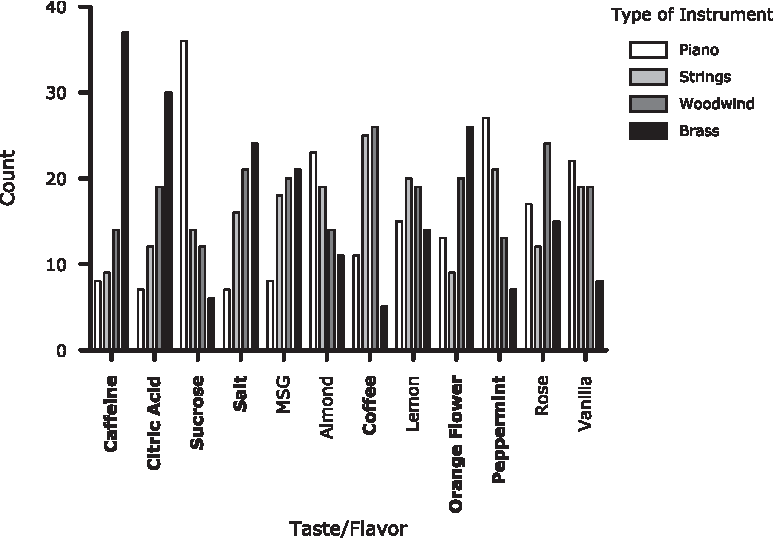
\includegraphics[width=0.8\textwidth]{figures/instr-taste}
    \caption[Musical instruments matched to the flavors]{Musical instruments matched to the flavors. Stimuli for which
    there were significant instrument preferences are marked with \emph{boldface} \citep{Crisinel2010}.}
    \label{fig:instruments}
\end{figure}

You can also adjust the size and the placement of the figure. \cref{fig:instruments} has its width set to 80\% of the
text width. While \LaTeX{} likes to determine the placement on its own, you can express your preference via the
parameters in \verb|\begin{figure}[placement]|. You can use \verb|h| (\emph{here} -- \LaTeX{} will try to place
the figure at the corresponding place or somewhere close), \verb|t| (\emph{top} -- the figure will be glued
to the top of the page), \verb|b| (\emph{bottom} -- bottom of the page) and any combination of them, while the order
determines the priority. If you get desperate, you can additionally use \verb|!|, which will try to force \LaTeX to
comply; however, sometimes even that can be unsuccessful; in that case, try to move figure to different places and
sections.

\subsection{Tables}
\label{sec:tables}

This template uses the \emph{booktabs} table style, which avoids vertical lines and uses horizontal lines sparingly
to make the tables cleaner. Similar to the \verb|figure| environment, you can define the tables via the \verb|table|
environment with the same system of positional parameters.

Inside, the \verb|tabular| environment defines the actual table: \verb|\begin{tabular}{lll}| in the case of
\cref{tab:example} declares a table with three columns aligned to the left (you can also use \verb|c| for centering,
and \verb|r| for the alignment to the right). In the table, you separate the columns with \verb|&| and lines
with \verb|\\|; any spacing around is ignored. You usually do not need to input a table manually, as there are many
web tools able to generate it for you from any kind of table format (e.g.,
\emph{\href{https://www.tablesgenerator.com/}{this one}}).

\begin{table}[htb]
    \centering
    \caption[An example table]{An example table. Notice that we place table captions above the table,
    whereas figure captions go below. Same as with figures, you can define a short name here as well.}
    \label{tab:example}
    \begin{tabular}{lll}
        \toprule
        \textbf{Participant} & \textbf{Age} & \textbf{Condition} \\
        \midrule
        P01                  & 22           & Control            \\
        P02                  & 25           & Experimental       \\
        P03                  & 21           & Control            \\
        \bottomrule
    \end{tabular}
\end{table}

\subsection{Algorithms}
\label{sec:algs}

If your thesis involves pseudocode of some algorithms, you can typeset it using the \verb|algorithm| environment
provided, in our case, by the \texttt{algorithm2e} package,
\footnote{For more details on the usage of this package, see \emph{
\href{https://www.overleaf.com/learn/latex/Algorithms\#The\_algorithm2e\_package}{this tutorial}}.}
which has been already configured for this template. As with any pseudocode, you are free to use any combination
of natural language, math notation, and programming elements to communicate the idea as efficiently and clearly as
possible.

Same as with the previous floating environments, the \verb|algorithm| environment works the same in terms of the
placement, captions, and labeling. If you use this environment anywhere in your document, the List of Algorithms
will be generated; otherwise, it stays hidden.

\begin{algorithm}[htb]
    \caption{Finding the maximum element in a sequence}
    \label{alg:maximum}

    \DontPrintSemicolon

    \KwIn{A finite sequence of numbers $A = \{a_1, a_2, \dots, a_n\}$}
    \KwOut{The maximum element in the sequence}

    \BlankLine

    $max \gets a_1$\;
    \For{$i \gets 2$ \KwTo $n$}{
        \If{$a_i > max$}{
            $max \gets a_i$\;
        }
    }
    \Return{$max$}\;
\end{algorithm}


